\section{Materiales Conductores}

Se llama conductores a aquellos materiales que poseen cargas libres de moverse en su volumen. Las carga se desplazan al aplicarse un campo eléctrico, las positivas en el sentido del campo y las negativas en sentido opuesto.

Si un conductor siente un campo eléctrico externo $\Vec{E_{ext}}$, sus cargas se desplazarán, formando polos positivos y negativos producto de los cuales se genera un campo eléctrico inducido dentro del material. El campo eléctrico total en el conductor es la suma del campo externo y el inducido.

\[\Vec{E} = \Vec{E}_{ext}+\Vec{E}_{ind}\]

\subsection{Equilibrio Electroestático}

Un conductor está en equilibrio electroestático cuando no presenta movimiento de cargas. En este estado se verifica que:

\begin{itemize}
    %Agregado relación entre E_ind y E_ext
    \item El campo eléctrico al interior del conductor es nulo, $\Vec{E}_{ind} = -\Vec{E}_{ext}$
    \item La carga neta al interior del conductor es nula, $\rho = 0$
    \item Sólo las superficies del conductor pueden poseer carga no nula
    \item El campo eléctrico producto de la carga superficial es normal a la superficie
    \[\Vec{E}=\frac{\sigma}{\epsilon_o}\hat{n}\]
    \item El potencial en el conductor es constante 
\end{itemize}

\subsection{Energía}

Para un sistema formado por $n$ conductores con cargas $\{Q_k\}^n_{k=1}$ y potenciales $\{V_k\}^n_{k=1}$, la energía potencial electrostática es

\[U_e = \frac{1}{2}\sum^n_{k=1}V_kQ_k\]

\subsection{Conductores Huecos}

Para un conductor de carga $Q$ con un agujero en su interior en equilibrio electroestático, se tiene que

\[Q = \int_{S_I}\sigma_I\,dS\,+\int_{S_E}\sigma_E\,dS\]

Donde $S_I$ es la superficie interior y $S_E$ la exterior.

\subsubsection{Carga Interior}

Si en el interior del agujero hay una carga $q$, entonces $\sigma_I$ no es necesariamente uniforme mientras que $\sigma_E$ sí lo es, y se verifica que

\[\int_{S_I}\sigma_I\,dS = -q\]
\[\int_{S_E}\sigma_E\,dS=Q-\int_{S_I}\sigma_I\,dS = Q+q\]

\subsubsection{Carga Exterior}

Si hay una carga al exterior del conductor, $S_E$ apantalla el efecto de $\Vec{E}_{ext}$ sobre $S_I$, de forma de $\sigma_I = 0$. (Funciona como una jaula de Faraday)

\subsection{Condensadores}

Se denomina condensador a sistema compuesto por 2 conductores con carga de igual magnitud y signo opuesto tales que su forma y posición relativa son fijas. En un condensador con cargas $Q_A = Q$ y $Q_B = -Q$ con $Q>0$, dado que la geometría del sistema es fija, se verifica que $\Vec{E}$ es proporcional a $Q$ ($\Vec{E}\propto Q$), en consecuencia la diferencia de potencial, dada por

\[\Delta V = V_A-V_B=\int^A_B \Vec{E} \cdot d\Vec{r}\]

también es proporcional a $Q$. En este caso como $Q_A$ es positivo $V_A > V_B$, puesto que el potencial decrece en el sentido del campo eléctrico (de carga positiva a negativa), en el caso general en que se desconoce cual carga es positiva, se tiene $\Delta V = |V_A + V_B|$.

\subsubsection{Capacitancia}

Se define la capacitancia $C$ de un condensador como la constante de proporcionalidad entre $\Delta V$ y $Q$. Depende únicamente de los parámetros geométricos del problema.

\[C=\frac{Q}{\Delta V}\]

\subsubsection{Energía en un Condensador}

La energía potencial electrostática en un condensador está dada por

\[U_e = \frac{1}{2}Q\Delta V = \frac{1}{2}C(\Delta V)^2=\frac{Q^2}{2C}\]

\subsubsection{Condensadores en paralelo}
Una cantidad $n$ de condensadores se encuentran conectados en paralelo cuando están conectados por sus dos extremos.
\begin{figure}[H]
    \centering
    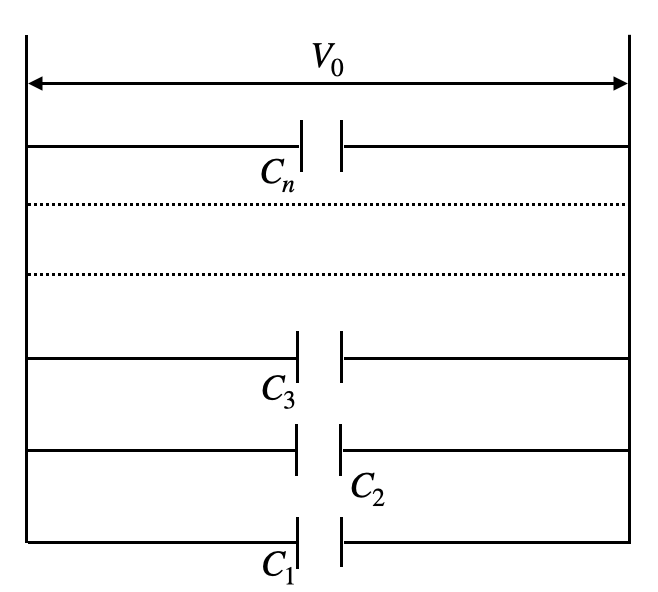
\includegraphics[width=0.42\textwidth]{Electroestática/conductores/condensadores_paralelo.png}
\end{figure}
Los condensadores en paralelo se pueden representar por un condensador equivalente con capacitancia $C_{eq}$, que viene dada por
\[C_{eq} = \sum_{i=1}^nC_i\]
A causa de que todos tienen la misma diferencia de potencial $\Delta V$.

\subsubsection{Condensadores en serie}
Una cantidad $n$ de condensadores se encuentran en serie cuando se conectar por 1 solo extremo entre sí.
\begin{figure}[H]
    \centering
    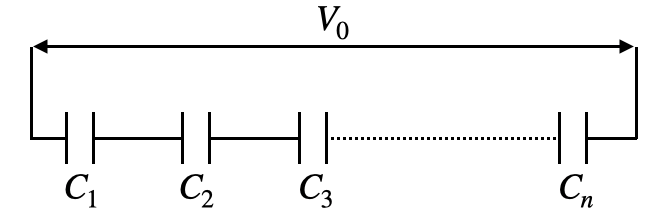
\includegraphics[width=0.55\textwidth]{Electroestática/conductores/condensadores_serie.png}
\end{figure}
Estos se pueden representar por un conductor equivalente con capacitancia $C_{eq}$, que viene dada por
\[C_{eq} = \left( \sum_{i=1}^n\frac{1}{C_i} \right)^{-1} \iff \frac{1}{C_{eq}} =\sum_{i=1}^n\frac{1}{C_i} \]
A causa de que la carga $Q$ es de igual magnitud en todas los conductores.

\newpage